\apendice{Código Fonte Arquivo Principal - defs}
	\index{C++}
	\index{\acs{uc}}
	O modelo tem suporte à C, C++, C\# e LaTeX para listings. Outras linguagens de programação são suportadas pelo pacote, mas os estilos não foram modificados. Os estilos são:

	\begin{itemize}
		\item customc
		\item cutomcs
		\item customcpp
		\item customlatex
	\end{itemize}

\apendice{Código Fonte Arquivo Principal - Estilo}
	\lstinputlisting[style=customlatex]{mymdt.sty}

\apendice{Código Fonte Arquivo Principal - root}
	\lstinputlisting[style=customlatex]{mdtRoot.tex}

\apendice{Arquivos de Fabricação - PCI do Protótipo}\label{app:gerbers}

	As Figuras \ref{img:gerbers:topbot}. Entradas no índice também podem ser incluídas nos apêndices. Por hora, os apêndices suportam somente um nível de referenciação (chapter). Futuras modificações visarão adicionar este suporte.
	\index{GERBER}
	\index{PCI}
	\index{GBL}
	\index{GTL}

	\begin{figure}[h]
		\caption{Camadas superior (azul), inferior (vermelho) e de corte (preto).}
		\label{img:gerbers:topbot}
		\centering
		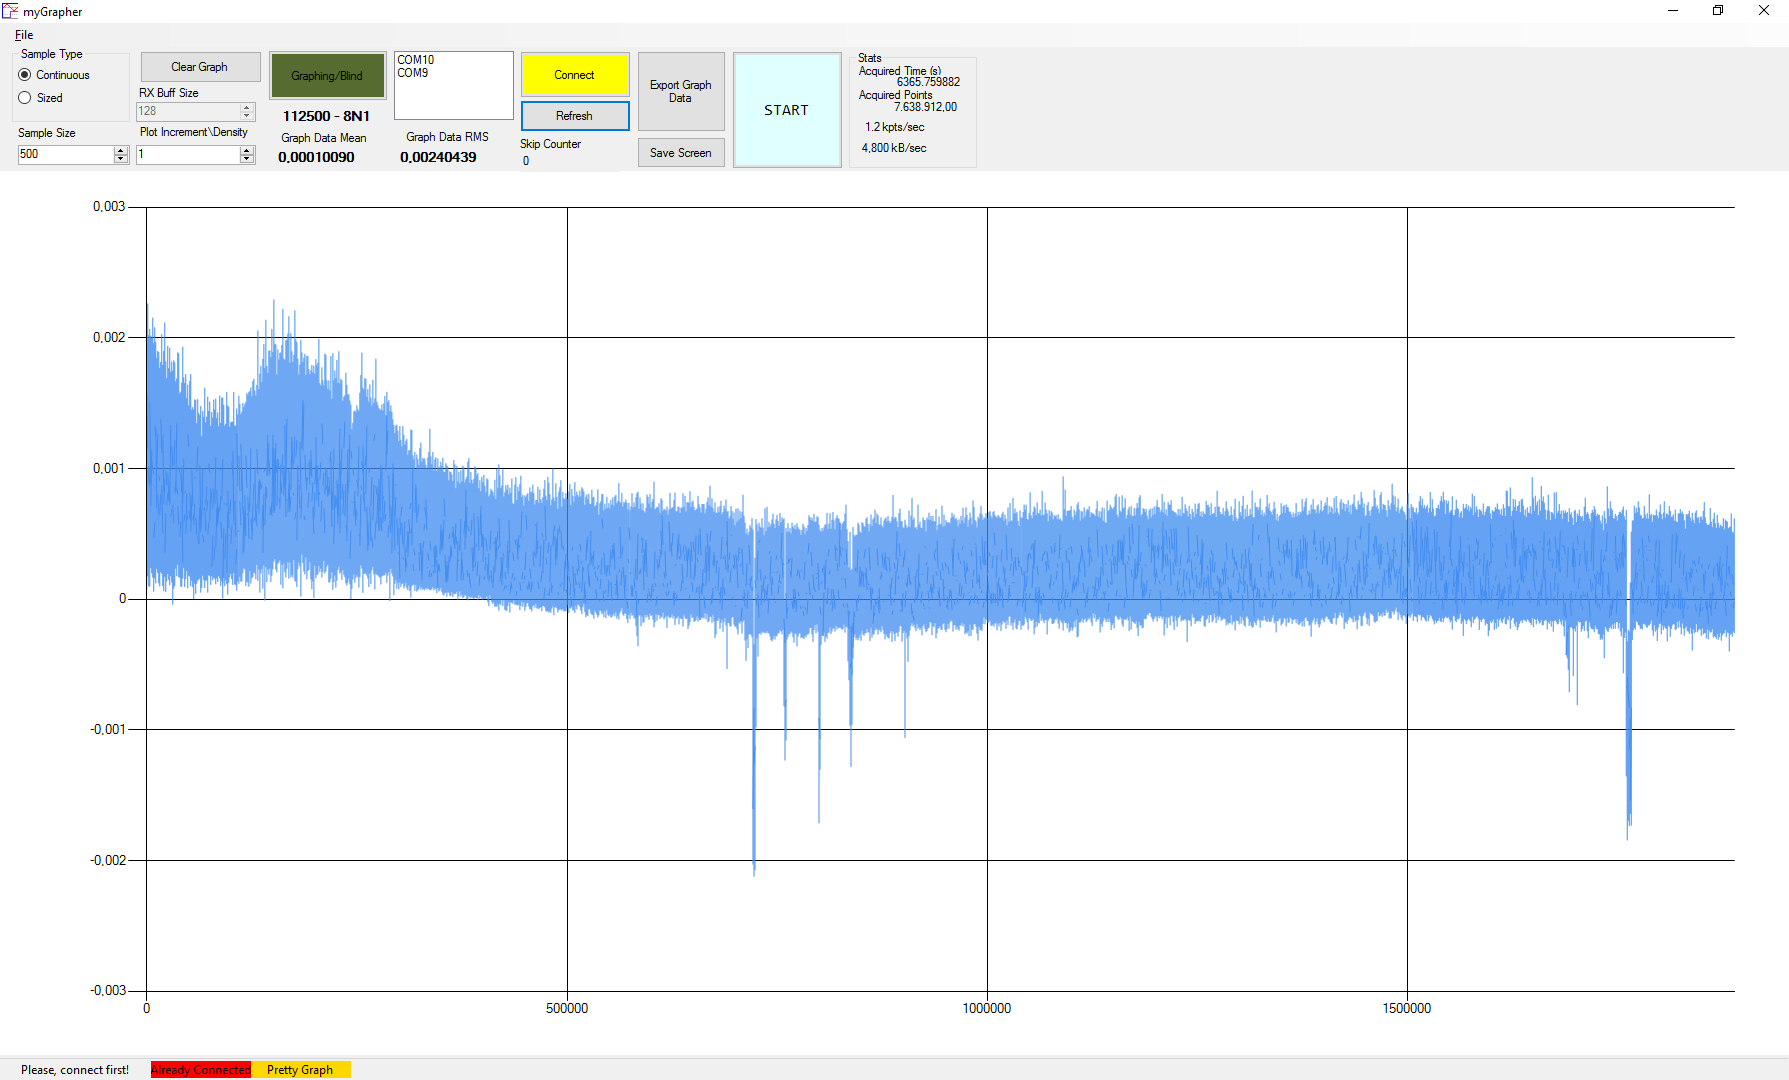
\includegraphics[width=0.3\linewidth,center]{images/appinaqcuisitionmode}
	\end{figure}
